\documentclass{gescons}

\genre {Atualizações}
\author{Paula Gabriella}
\authorrole{Voluntária do Setor de Comunicação da Editares}
\title{Projetos Digitais Modernizam a Comunicação Editorial da Editares}
%\roles{Voluntária do Setor de Comunicação da Editares}

\begin{document}
    \makeentrevistatitle
    %\maketitle

    %\fullwidthimage{fields}{b}

    %\coverart{back/editorial}
    \coverart{../fundo-generico.png}
    
    
\begin{center}
    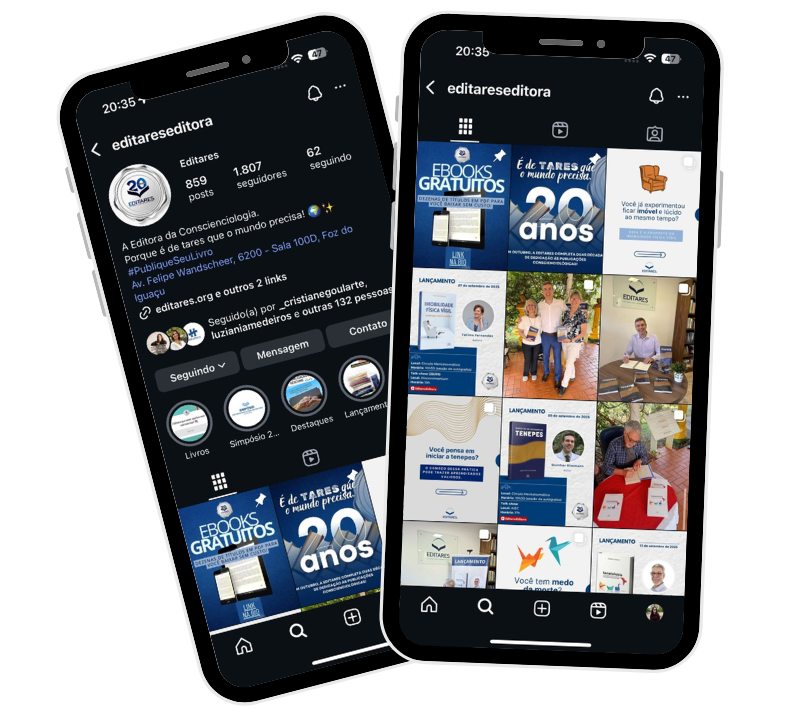
\includegraphics[height=10cm]{articles/atualizacoes/fotos/materia5/Instagram-Editares.png} 
\end{center}
    
    \begin{multicols}{2}


Nos últimos anos, a comunicação da Editares passou por importantes atualizações. O trabalho de divulgação não se restringe apenas ao anúncio de novos lançamentos, mas se dedica principalmente a valorizar e compartilhar os conteúdos de gescons publicadas. A proposta é \textbf{oferecer ao futuro leitor amostra prática} do que encontrará nas obras, ampliando o alcance de cada livro.

Nesse sentido, a Editares tem investido em diferentes formatos para tornar o conteúdo mais acessível e interativo. Entre eles, destacam-se os vídeos gravados pelos autores, que aproximam o leitor da vivência pessoal de quem escreveu a obra, e os carrosséis produzidos a partir das resenhas, que apresentam as ideias centrais de maneira visual e objetiva. Assim, cada publicação nas redes sociais se torna uma oportunidade para aprofundar a compreensão e estimular o interesse pela leitura.

Além disso, a Editares tem promovido \textbf{ações que fortalecem o vínculo entre os livros e a comunidade conscienciológica.} Dentre elas, destacam-se:

\begin{enumerate}
\def\labelenumi{\arabic{enumi}.}
\item
  Dicas de leitura associadas a cursos em andamento, criando conexões pertinentes para o aluno e favorecem a interação com as instituições parceiras;
\item
  Campanhas promocionais em datas especiais, como a promoção do livro Comunicação Evolutiva durante o aniversário de 20 anos da Comunicons.
\end{enumerate}

Essas iniciativas têm tornado a Editares mais presente e ampliado o alcance do conteúdo das gescons a um público cada vez maior. Ao divulgar trechos, ideias e reflexões dos livros, a Editares reforça seu papel como ponte entre o conhecimento conscienciológico e o leitor, promovendo a expansão da interassistência por meio da leitura.


% {[}INSERIR FOTO QUE ESTÁ NA PASTA MATÉRIA 5{]}


%\begin{center}
%    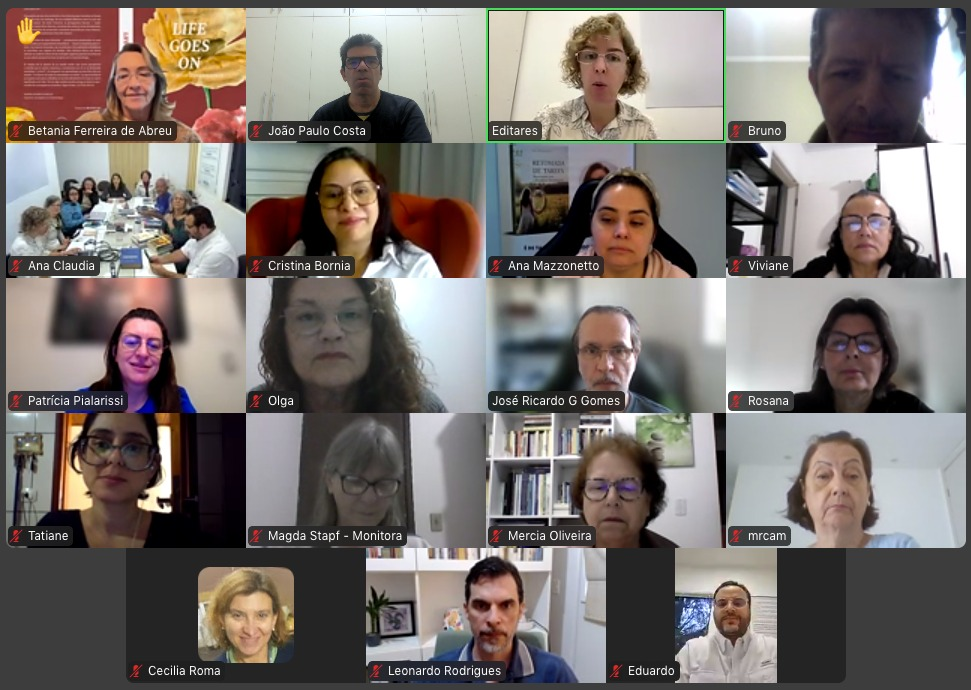
\includegraphics[width=9cm]{articles/atualizacoes/fotos/escola-editores/escola-editores1.jpeg} 
%\end{center}


    \end{multicols}
\end{document}

